\documentclass[class=article,border=5pt,tikz]{standalone}

\begin{document}
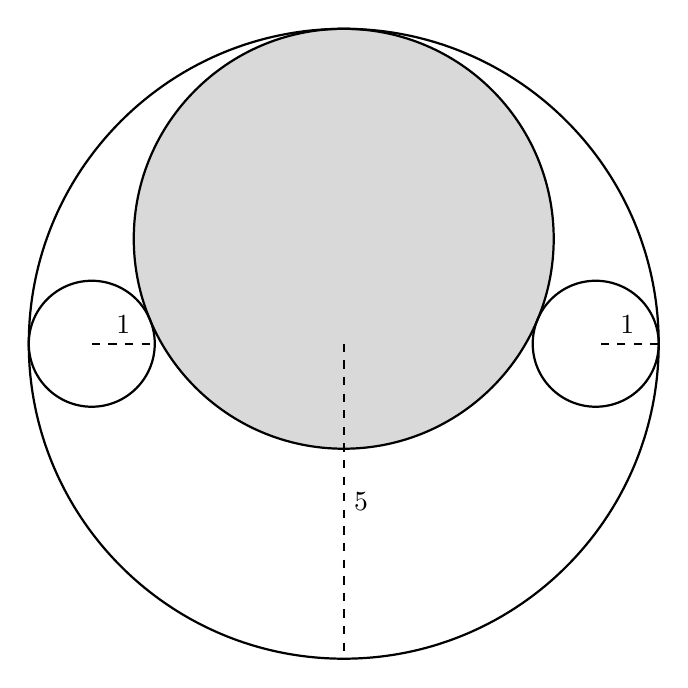
\begin{tikzpicture}[thick,x=0.8cm,y=0.8cm]
  \pgfmathsetmacro\x{5}
  \pgfmathsetmacro\y{3.33333}
  \pgfmathsetmacro\z{1}
  % larger of the inscribed circles:
  \draw[fill=gray!30] (0,\x-\y) circle (\y);
  % small inscribed circles:
  \draw (-\x+\z,0) circle (\z);
  \draw (\x-\z,0) circle (\z);
  % radius of small circles:
  \draw[dashed] (-\x+\z,0) --++ (\z,0) node[midway,above] {$1$};
  \draw[dashed] (\x,0) --++ (-\z,0) node[midway,above] {$1$};
  % large circle:
  \draw (0,0) circle (\x);
  % radius of large circle:
  \draw[dashed] (0,0) --++ (0,-\x) node[midway,right] {$5$};
\end{tikzpicture}


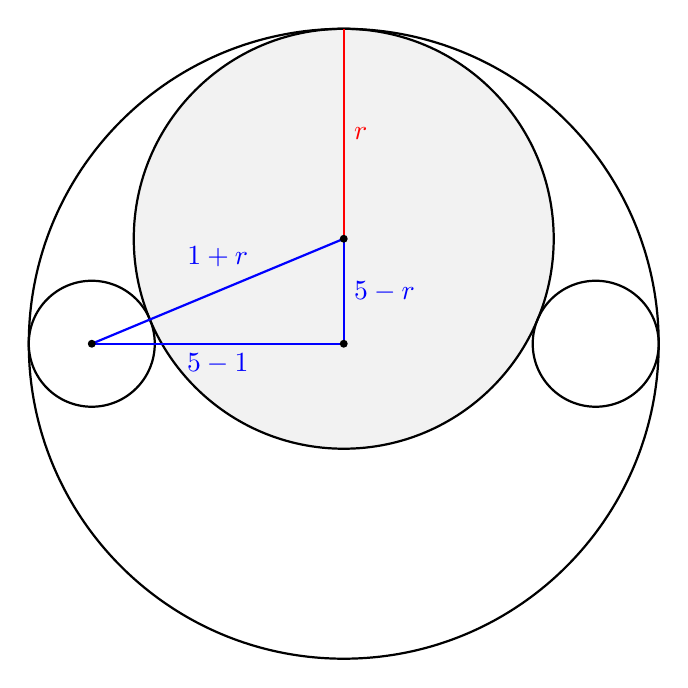
\begin{tikzpicture}[thick,x=0.8cm,y=0.8cm]
  \pgfmathsetmacro\x{5}
  \pgfmathsetmacro\y{3.33333}
  \pgfmathsetmacro\z{1}
  % larger of the inscribed circles:
  \draw[fill=gray!10] (0,\x-\y) circle (\y);
  % small inscribed circles:
  \draw (-\x+\z,0) circle (\z);
  \draw (\x-\z,0) circle (\z);
  % large circle:
  \draw (0,0) circle (\x);
  % hypotenuse of right triangle (combined radius of large and small circles):
  \draw[blue] (0,\x-\y) -- (-\x+\z,0) node[midway,above,yshift={5pt}] {$1+r$};
  % short leg of right triangle:
  \draw[blue] (0,\x-\y) -- (0,0) node[midway,right] {$5-r$};
  % long leg of right triangle:
  \draw[blue] (-\x+\z,0) -- (0,0) node[midway,below] {$5-1$};
  % radius of shaded circle:
  \draw[red] (0,\x-\y) --++ (0,\y) node[midway,right] {$r$};
  % mark center of circles:
  \draw[fill=black] (0,0) circle (1pt);
  \draw[fill=black] (0,\x-\y) circle (1pt);
  \draw[fill=black] (-\x+\z,0) circle (1pt);
\end{tikzpicture}

\end{document}


